\documentclass[conference,10pt]{IEEEtran}


\usepackage{amssymb}
\usepackage{amsmath}
\usepackage{algorithm}
\usepackage{algorithmic}
\usepackage{graphicx}
\usepackage{cite}
\usepackage{array}
\usepackage{cases}
\usepackage{booktabs}
\usepackage{multirow}
\usepackage{epsfig}
\usepackage[TABBOTCAP]{subfigure}

\setlength{\columnsep}{0.25in}
    
\newtheorem{definition}{Definition}
\newtheorem{theorem}{Theorem}
\newtheorem{proposition}{Proposition}
\newtheorem{corollary}{Corollary}
\newtheorem{lemma}{Lemma}
\newtheorem{remark}{Remark}
\newtheorem{problem}{Problem}

\hyphenation{op-tical net-works semi-conduc-tor}

\hyphenpenalty=5000
\tolerance=1200
\newcommand{\pName}{AWE}  
\newcommand{\sysname}{\emph{Encounternet}} 


\begin{document}

\title{{\pName}: A Mac-Layer Encounter Protocol for a Wildlife Tracking System}



\maketitle

\begin{abstract}
Encounters between wild animals mark of the same or different species mark important events, such 
as mating, predation, and disease contraction, and they define the social structure of animal groups.
Several real-world systems designed to record such encounters have been implemented in the wildlife-research community.
In these systems, energy-restricted short-range radio devices are attached to wild animals, transmit identification
packets periodically, and receive and record packets from others.
%    Encounters are common interactions of wild animals.
%    Several real encounter-registration systems have been implemented
%    to help record the encounter process. In these systems, wild animals
%    are attached with energy-restricted radio devices called tags, 
%    to transmit packets periodically
%    and record the encounter process with others.
    However, non-trivial protocols for this problem have not been studies, and neither did the
    fundamental tradeoff 
    between minimizing the power consumption 
    and reducing the encounter latency. Our insight is that it is reasonable for a tag to
    increase the working frequency of its radio when encounter happens, and otherwise keeps
    the radio in a low-power mode. The key is to design a mechanism
    to identify the existence of an encounter in real-time. 

    In this paper, we propose a robust encounter registration protocol that with 
    high probability accomplishes the encounter registration 
    in $O(k)$ slots time, assuming $k$ is the number of encounter tags.
    Our protocol consists of two process: detect other tags with low energy consumption; 
    and make connections with the detected tags to record each other's ID. 
    We analyze the performance of this protocol under a formulated radio model and carry out a number of
    experiments to validate this model.
    To the best of our knowledge, this is the first practical protocol for a real 
    encounter-registration system.

\end{abstract}



\section{Introduction}

Collecting detailed information about wild animals~\cite{Prangle2006NewRadiocolars,Rutz2012AutomatedMapping} 
remains a significant technical challenge that
limits the ability of Ecologists to study them, the interactions between them, and the interactions 
between wild animals and their environment. One tools that has emerged a little over a decade ago
and has been gaining significance is 
{\em encounter detection and logging}~\cite{Tentelier2016FishNetwork,
Bohm2009WildlifeLivestock,Ripperger2016ProximitySensing}.

Encounter detection systems~\cite{Levin2015Performance,Menhill2012NovelTelemetry,dressler2016bats} 
consist of radio devices called {\em tags} that are attached to wild
animals (and sometimes also to fixed positions and to livestock), as depicted in Fig.~\ref{tags}. 
The radios transmit identification
packets periodically, usually once every few seconds. The radios also listen to such packets, not
necessarily continuously, and record data about received packets in persistent memory on the tag. The
radios are typically configured for short-range communication by using low transmit power and by 
using high data-rates (both limit the signal-to-noise ratio at the receiver). Because the radios
are configured for short-range communication, receiving a packet implies that the transmitting tag is
in close proximity to the receiving tag. Recent systems record with each packet a received signal strentgh
indication (RSSI)~\cite{Daiya2011Experimental}, which helps to estimate the distance between the transmitter and receiver.
This is the main goal of these systems: to log close-proximity
events between two or more animals. The logs are downloaded either by physically retrieving the tags,
or remote download to base-stations placed in locations that the animals are known to frequent.

Such systems have gained popularity among Ecologists because the tags are relatively inexpensive and can
be very small, because deployment does not require much infrastructure in the field, and because close-proximity
encounters are key aspects of many significant events in the life of animals: mating, predation, transmission of infectious
diseases, and so on. We comment on some of these applications in Section~\ref{sec:related-work}.

\begin{figure}[!t]
    \centering
    \includegraphics[width=3in]{figures/tag}
    \caption{Printed circuit boards for Encounternet tags~\protect\cite{Menhill2012NovelTelemetry}.
    Lines are 5mm apart. Complete tags require the addition of miniature batteries, whip antenna, and
    coating. The small batteries make effective protocols important.}
    \label{tags}
\end{figure}

Encounter-registration systems pose challenging protocol-ralated problems. One problem is to minimize
the power used for listening to other tags. All of the systems developed so far have used low-power integrated
UHF transceivers, and the power consumed by these while receiving is comparable to the power that they use
to transmit. The dominant strategy to address this issue appears to be duty-cycling the 
receiver~\cite{Zhang2017Performance}, so that it is
off most of the time. Synchronizing the timing of the activity periods of all tags can minimize total receive energy
while maximizing that transmissions will be received. If tags do not synchronize their activity periods, many transmissions
at close proximity may go unnoticed; this is not an unreasonable solution if encounters are long. Another emerging approach
to the receive-power problem is based on so-called {\em wake-up receivers}, specialized nano-power sub-receivers whose only
job is to wake up the main receiver when a strong packet is received. These have not been used in Ecology research so we
exclude them from most of the discussion; we do comment on them in Section~\ref{sec:related-work}.

The other protocol-related problem is interference. 
If many tags transmit simultaneously, receiving tags may fail
to reconstruct valid packets. Paradoxically, highly-efficient 
systems with good time synchronization and short activity
periods suffer more from this problem than less efficient systems 
in which the clocks of tags are not synchronized tightly
enough to transmit simultaneously. This is not a theoretical problem; 
many species of animals, including many species of
birds and bats, roost together, so encounters of tens or hundreds 
of individuals are not necessarily rare.

Our fundamental observation is that it is a waste of 
energy if an animal is not encountering with others
while still keeps the tag working frequently.
Thus it is reasonable for a tag to
increase the working frequency of its radio when 
encounter happens; otherwise it keeps
the radio in a low-power mode. The key is to design a mechanism
to identify the existence of an encounter in real-time. 



In this paper, we propose an effective protocol for encounter registration, 
addressing these two problems systematically and
methodically. In our protocol, we design two stages for the tags, 
namely detecting stage and connecting stage.
In the detecting stage, a tag works a fraction of time in order to save energy,
and transmits a beacon periodically to detect whether an encounter is happening at the moment.
When detected an acknowledgement, the tag switches to the connecting stage and increases the 
transmission frequency in order to establish links with other tags. To deal with interference 
caused by 
In the connecting stage,
a tag adaptively adjusts its transmission probability: it increases the probability when 
the channel is detected idle and reduces the probability when interference is detected.  


We present concrete analysis of the protocol under our radio model
and carry out a number of experiments to validate this model.
We prove that our protocol accomplishes the encounter registration
of $k$ tags in $O(k)$ slots time.


%% Remaining structure
The remainder of the paper is organized as follows. 
The next section highlights the related works.
Section~\ref{sectionmodel} presents the system model and basic definitions.
We present the concrete protocol design
in Section~\ref{sectionprotocol}. We  
analyze the performance of our protocol in Section~\ref{sectionanalysis}. 
We validate the radio model by real experiments in Section~\ref{sectionsimulation}, 
and the paper is concluded in Section~\ref{sectionconclusion}.

% \section{Background and Related Work}
\label{sectionbackground}

% \newcommand{\pName}{anminal} 

\subsection{System background}

{\sysname}~\cite{Levin2015Performance}



\section{Related Work}
\label{RW}




\section{System Model}
\label{sectionmodel}

In this paper, we study the encounter problem in a wildlife 
tracing system. 
We call individual animals as \emph{agents}, 
and \emph{peers} are referred as other agents that distinguish from 
a specific one.
The definition of the \emph{Encounter process} is formulated as follows.
\begin{definition}
Encounter is defined as the process that 
an agent detects and records message
from other peer(s) if they keep at least $T_0$ slots of 
close proximity $\Delta \leq D$
in the wildlife tracking system. 
\end{definition}

In the following, we describe the system model for theoretical analysis in this paper.



\subsection{Communication Model}

% First, we present the communication model in this paper.

In the  wildlife tracing system {\sysname}, the encounter process 
is a common biological behavior and
happens when more than one agents gather closely, constituting a 
single clique of size $k$~($k \geq 2$).
Note that, $k$ is not known to each agent and the whole 
clique composes a sing-hop network for communication due to the proximity. 

Each agent is equipped with a tag containing radio. 
An agent that has its radio on can choose to be in the $Transmit$ state
or the $Listen$ state:
\begin{itemize}
\item \textbf{Transmit state:} an agent transmits (broadcasts) 
a message containing its ID on the channel;
\item  \textbf{Listen state:} an agent listens on 
the channel to receive messages from peers.
\end{itemize}

Suppose time is divided into slots of equal length $t_0$
, which is assumed to be sufficient to finish a complete
communication process (one agent transmits a message including its ID and
a peer receives the message).

An agent transmit successfully in a time slot if and only if 
it is the only one transmitting and all the other peer(s) will
receive its message and record its ID. Otherwise the channel is detected
as \emph{idle} if there is no transmission and \emph{busy} if there 
are simultaneous messages.

In the wildlife tracing system {\sysname}, 
on the one hand,
each agent (animal) is equipped with an energy-restricted tag;
on the other hand, encounter process happens occasionally, and
it is a waste of energy if transmitting while there is no encounter with other peer(s). 
Thus in order to keep a balance between the energy consumption 
and the efficiency of encounter process, we introduce the duty cycle mechanism.

\textbf{Duty cycle mechanism.} 
An agent has the capability to turn off the radio to save
energy for most of the time, and may only be active 
(transmitting or receiving) during a fraction $\theta$ of the time.
%, where $\theta$ is typically $1/100$ or less.

Incorporating the duty cycle mechanism, in each time slot an agent $u_i$ is able to adopt an action as:
$$ s_i^t=\left\{
\begin{aligned}
&Sleep  & & & &{sleep~ with~ probability~ (1-\theta_i)}  	 \\
&Transmit  & & & &{transmit~ with~ probability~ \theta_i p}	\\
&Listen  & & & &{listen~ with~ probability~\theta_i(1-p)}	\\
\end{aligned}
\right.
$$
\emph{Duty cycle} is defined as the fraction of time an agent turns its radio on, 
which is formulated as:
$$\theta_i=\frac{|\{t: 0\leq t<t_0, s_i(t) \in \{Transimit,Listen\}\}|}{t_0}.
$$

% \subsection{Interference Model}

% In reality, wireless transmission suffers from interference.
% We consider graph model as the interference model in our protocol. 
% Graph model is a popular one that enables the development of
% efficient algorithms for crucial networking problems. Some other models,
% such as the signal to interference plus noise ratio (\emph{SINR}) model,
% are more complicated and lack good algorithmic features. 
% In addition, it is shown that SINR can be transformed to the graph model by
% particular means.

% In the graph model, we assume that the communication range of each agent 
% is $D$ meters and an agent $u_i$ can discover its nearby peer $u_j$ 
% in time slot $t$ if and only if $u_j$ is the only peer in $u_i$'s range 
% that transmits and $u_i$ is listening in the slot.




% Suppose the distance between two nodes $u_i$ and $u_j$ is $\Delta_{i,j}$.
% The connectivity of the edge $e_{i,j}$ in the graph model is formulated as:
% $$ \omega_e=\left\{
% \begin{aligned}
% &0  & & &   &D \leq \Delta_{i,j}	 \\
% %&\phi_{i,j}  & & & 	&d \leq \Delta_{i,j} \leq D\\
% &1  & & & &\Delta_{i,j} \leq D	\\
% \end{aligned}
% \right.
% $$
% %where $\varphi(\Delta)$ is an inverse function 
% %(e.g., the weight is inversely proportional to the distance).
 
% An agent $u_i$ can discover its peer $u_j$ in
% time slot $t$ if and only if $u_j$ is the only peer transmitting 
% in the range of $u_i$ ($\Delta_{i,j} \leq D$) and $u_i$ is listening in the slot.
% An agent suffers from collisions when it receives simultaneous messages. 


\textbf{Collision detection mechanism.}
A listening agent can distinguish whether the channel is \emph{idle} or \emph{busy}, 
apart from successful receiving a message. 

\subsection{Problem formulation}

We formulate the problem in this paper as follows:
\begin{problem}
    We define an encounter problem as to design a protocol to guarantee 
    all the agents in the clique can receive message from each other at least once 
    if they encounter for at least $T$ ($T \leq T_0$) time 
    slots~(i.e., $T$ is the upper bound of the protocol). 
\end{problem}


We look into the problem and find the key challenge is 
the uncertainty of dynamic movements
of agents. Despite the dynamicity in this real system, 
when $T_0$ is short enough relative to 
the time required for an agent to move a step~(a short distance)
in reality~(e.g., less than $1$ second),
we can make a reasonable assumption that the communication 
connectivity of the agents is stable during each $T_0$ time slots. 



\section{Adaptive Wildlife Encounter protocol}
\label{sectionprotocol}

In this section, we present our Adaptive Wildlife Encounter~(AWE) protocol.
The pseudo-code of the protocol is given in Algorithm~\ref{DA} and Algorithm~\ref{CA}.

{\pName} consists of two stages: detecting stage and 
connecting stage. 
\begin{itemize}
    \item \textbf{Stage 1: detecting stage.} In this stage, an agent attempts to
    detect whether there are nearby peers, regardless of who they are. 
    \item \textbf{Stage 2: connecting stage} In this stage, an agent attempts to 
    identify the nearby peer(s) and record their IDs to its log.
\end{itemize}

Initially, each agent starts from the detecting stage. 
In the detecting stage, an agent turns its radio to the $sleep$ state most of the time,
and switches to $transmit$ state or $listen$ state at intervals.
In the connecting stage, agents only switch between $transmit$ state 
and $listen$ state.

The key idea of {\pName} is that, any single agent keeps in detecting 
stage to reduce ineffective energy consumption. When encounter happens, 
it detects the existence of nearby peers and turns to the connecting stage 
to identify those peers (or a peer) as fast as possible and record the encounter process to its log. 
when the encounter process is determined to be finished in the connecting stage, 
the agent turns back to the detecting stage.

\begin{remark}
    In the {\pName} protocol, there is no need to synchronize the stage between agents and
    {\pName} still works when encounter peers are in different stage, e.g., an agent in detecting 
    stage bursts into a stable clique in connecting stage. 
    The proof of correctness will be presented 
    in section~\ref{sectionanalysis}. 
\end{remark}

In the following, we describe the operations of these two stages in detail. 

\subsection{Detecting stage}

In the detecting stage,  
energy efficiency is achieved by the duty cycle mechanism, 
e.g., denote the predefined duty cycle for 
all the agents is $\theta$, the tag radio of each agent will work
$\theta T_0$ slots in every period of $T_0$ slots. 

However, it is very ineffective
when two agents encounter and one is in $sleep$ state while the other is transmitting
or listening. 
To technically achieve synchronizing the time that agents turn on the radio without extra cost,
we introduce the technique of Relax Difference Set (RDS)~\cite{luk1997two}.
We use the RDS technique to guarantee that every encounter pair 
of agents turn on the radio in the same slot at least once in each round $T_0$.

RDS is an efficient tool to construct cyclic quorum systems. 
The definition is:
\begin{definition}
A set $R=\{a_1,a_2,...,a_k\} \subseteq Z_T$ (the set of all non-negative integers less than $T$)
is called a RDS if for every $d \neq 0$ (mod $T$),
there exists at least one ordered pair $(a_i,a_j)$ such that $a_i - a_j \equiv d$ (mod $T$), 
where $a_i,a_j \in D$.
\end{definition}

\begin{figure}[h]
    \centering
    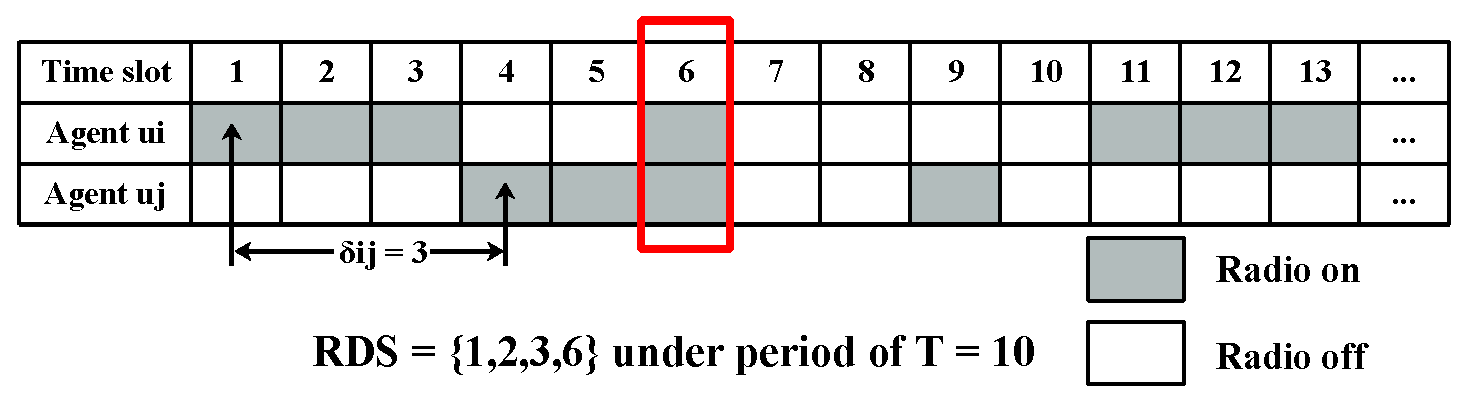
\includegraphics[width=3.5in]{figures/RDS}
    \caption{A example of how RDS works to help synchronization. Consider a period
    of $ten$ slots and the time drift between two agents $u_i$ and 
    $u_j$ is $3$. There exists an ordered pair $(6,3)$ in the constructed RDS such that $6 - 3 \equiv 3$ (mod $10$). Thus 
    they will determinately turn on the radio at the same slot in every period $T$, 
    which is the $6^{th}$ slot in a period of $u_i$ and the $3^{th}$ slot in that of $u_j$ respectively.}
    \label{exampleRDS}
\end{figure}

We now give an example to explain how RDS works to help synchronization.
Suppose the duty cycle is set as $0.4$, i.e., there are $4$ active slots 
in every $10$ slots. It is easy to show that $R=\{1,2,3,6\}$ is a RDS
under $Z_{10}$:
\begin{align*}
    &2 - 1 = 1,\quad 3 - 1 = 2,\quad 6 - 3 = 3,\quad 6 - 2 = 4, \\
    &6 - 1 = 5,\quad {2 - 6 = 6}~{(mod~10)},\quad \dots,\quad \dots, 
\end{align*}
In every period of ten slots, for any $i = \{0,1,\dots,9\}$, if $i \in R$, then
the agent turns on its radio in the $i^{th}$ slot in this period; otherwise it turns off the 
radio to the $sleep$ state. An example is depicted in Figure~\ref{exampleRDS}. 



\begin{algorithm}[!h]
    \caption{RDS Construction Algorithm}
    \label{RDS}
    \begin{algorithmic}[1]
    \STATE $R :=\emptyset$; $\lambda :=\lceil \sqrt{N}  \rceil$,
    $\mu :=\lceil \frac{\lceil \sqrt{N} \rceil}{2} \rceil$;\label{RDSline1}
    \FOR{$i = 1 :\lambda$}
        \STATE $R :=R \cup i$; \label{RDSline2}
    \ENDFOR
    \FOR{$j = 1 :\mu$}
        \STATE $R :=R \cup (1 + j * \lambda )$; \label{RDSline3}
    \ENDFOR
    \end{algorithmic}
\end{algorithm}

It has been proved that any RDS must have cardinality $|R| \geq \sqrt{N}$\cite{luk1997two}.
We present a linear algorithm to construct a RDS with 
cardinality $\lceil \frac{3\sqrt{T_0}}{2}  \rceil$ under $Z_{T_0}$ in Alg. \ref{RDS}.

We show the correctness of the construction formally.
%The correctness proof of the construction
\begin{lemma}
\label{RDS1}
Set $R = \{r_0, r_1, ..., r_{\lambda + \mu - 1}\}$ constructed in Alg. \ref{RDS} is a RDS,
where $|R| = \lambda + \mu = \lceil \sqrt{T_0}  \rceil + \lceil \frac{\lceil \sqrt{T_0} \rceil}{2} \rceil
\approx \lceil \frac{3\sqrt{T_0}}{2}  \rceil$.
\end{lemma}
\begin{IEEEproof}
Obviously, if there exists one ordered pair $(a_i,a_j)$ satisfying  $a_i - a_j \equiv d$ (mod $T_0$),
an opposing pair $(a_j,a_i)$ exists such that
$a_j - a_i \equiv (T_0-d)$ (mod $T_0$). Thus we only need to find
at least one ordered pair $(a_i,a_j)$ for each $d \in [1, \lfloor T_0/2 \rfloor]$.

In the construction, $\lambda$ in Line \ref{RDSline1} is the smallest integer satisfying
$\lambda^2 \geq T_0$. Every $d$ in range $[1, \lfloor T_0/2 \rfloor]$
can be represented as: $ d = 1 + j \times \lambda - i$, where $1 \leq j \leq \mu,
1 \leq i \leq \lambda$. Thus, there exists $a_j = 1 + j \times \lambda$
from Line. \ref{RDSline2} and $a_i = i$ from Line. \ref{RDSline3}
satisfying  $a_j - a_i \equiv d$. Then, the lemma can be derived.
\end{IEEEproof}

\begin{algorithm}[!h]
    \caption{Detecting Algorithm}
    \label{DA}
    \begin{algorithmic}[1]
    \STATE $T_0 := \lceil \frac{9}{4\theta^{2}} \rceil$; $\omega_0 :=\frac{1}{2}$; $t := 0$;
    \STATE Invoke Alg.~\ref{RDS} to construct $R = \{r_0, r_1, ...,r_{\lceil 
    \frac{3\sqrt{T_0}}{2}  \rceil}\}$ under $Z_{T_0}$;
    \WHILE {$True$}
        \IF{$(t + 1) \in R$}  \label{On}
            \STATE \textbf{\emph{In the first sub-slot:}}
            \STATE Transmit a beacon with probability $\omega_0$
            and listen with probability $1-\omega_0$;
            \STATE \textbf{\emph{In the second sub-slot:}}
            \IF{the agent is in $listen$ state in the first sub-slot}
                \IF{detects~energy~(a~beacon~or~a~collision~by~multiple~beacons)~in~the~first~sub-slot}
                    \STATE Transmit a beacon and turn to the \textbf{connecting stage};
                \ENDIF
            \ELSIF{detects~energy~(a~beacon~or~a~collision~by~multiple~beacons)~in~this~sub-slot}
                \STATE Turn to the \textbf{connecting stage};
            \ENDIF
        \ELSE
                \STATE $Sleep$ in the whole slot;
        \ENDIF
        \STATE $t := (t + 1) \% T_0$;
    \ENDWHILE
    \end{algorithmic}
\end{algorithm}

Based on the RDS, we present the operations in the detecting stage as Alg.~\ref{DA}.
Each slot is divided into two sub-slots.
Agents turn on and off the radio according to the RDS sequence,
Consider a slot the radio is on. In the first sub-slot
an agent transmits a beacon with probability $\omega_0$ and listens with probability $(1-\omega_0)$.
In the second sub-slot: 
\begin{itemize}
    \item[1)] The agent is in $listen$ state in the first sub-slot:
    \begin{itemize}
    \item if the agent detects a beacon (or beacons) in the first sub-slot, it 
    transmits a beacon (a bit is OK) as an acknowledgement 
    on the channel in the second sub-slot and turn to the 
    connecting stage; otherwise it does nothing. 
    \end{itemize}
    \item[2)] The agent is in $transmit$ state in the first sub-slot:
    \begin{itemize}
    \item if the agent detects a beacon (or beacons) in this sub-slot,
    it turns to the connecting stage; otherwise it does nothing.
    \end{itemize}
\end{itemize}

As discussed before, the aim of this stage is to detect nearby peer(s) as fast as possible 
(if exists), and either successful transmission or detecting busy on the channel activates the agent
to switch to the connecting stage. Hence we fix the transmitting probability as $\omega_0 = \frac{1}{2}$. 

% \begin{remark}
%     Though $\omega_0 = \frac{1}{2}$ is not the optimal probability in multi-agent encounter cases, 
%     the probability that an agent detects a peer in a slot grows as the number of agents
%     increases. This is because a new agent will not interrupt but help other agents to detect peers
%     if it is in $transmit$ state in a slot.
% \end{remark}

\subsection{Connecting stage}

In the connecting stage, agents attempt to identify the nearby 
peers and record the encounter to its log.
A successful identification happens only if the agent is listening
and exactly one peer is transmitting. 

\begin{algorithm}[ht]
    \caption{Connecting Algorithm}
    \label{CA}
    \begin{algorithmic}[1]
    \STATE $t := 0$; $\omega_t := \zeta$; 
    \WHILE {$True$}
        \STATE \textbf{\emph{In the first sub-slot:}}
        \STATE Transmit a message containing ID with probability $\omega_t$
        and listen with probability $1-\omega_t$;
        \STATE \textbf{\emph{In the second sub-slot:}}
        \IF{the agent is in $listen$ state in the first sub-slot}
            \IF{reveive a message successfully}
                \STATE Record the source ID and transmit a beacon;
                \STATE Set $\omega_{t+1} := \frac{\omega_t}{(1+\epsilon)}$;
            \ELSIF{channel is idle}
                \STATE Set $\omega_{t+1} := min\{(1+\epsilon)\cdot\omega_t, \zeta\}$;
            \ELSE
                \STATE Set $\omega_{t+1} := \frac{\omega_t}{(1+\epsilon)}$; $\backslash\backslash$ the channel is busy
            \ENDIF
        \ELSE
            \IF{detect beacons in this sub-slot}
                \STATE $\omega_{t+1} := 0$;
            \ELSE
                \STATE Set $\omega_{t+1} := \frac{\omega_t}{(1+\epsilon)}$;
            \ENDIF
        \ENDIF
        \STATE $t := (t + 1)$;
        \IF{$t == \hat{T}$}
            \IF{no peer is found in this round}
                \STATE Turn to the \textbf{detecting stage}; \label{backDS}
            \ELSE
                \STATE $t := 0$; $\omega_t := \zeta$;
            \ENDIF
        \ENDIF
    \ENDWHILE
    \end{algorithmic}
\end{algorithm}



The collision detection (CD) mechanism is incorporated in this stage 
to increase of efficiency. This mechanism enables the listening agent 
to notify the transmitting peers of the transmission outcomes, 
and thus they take measures to reduce the collisions if not successful.

In this stage, every $\hat{T}$ slots consists of a round. Each 
agent repeats the operations in Alg.~\ref{CA} round by round and 
it turns to the connecting stage when it cannot find any peer in a complete round, 
as the operation in Line~\ref{backDS}.

As discussed in section~\ref{sectionmodel}, $\hat{T}$ is relatively short in 
real world, thus the communication connectivity stays stable in a round. 
However, due to the dynamic movements of agents, the communication connectivity
may change from round to round, so all the parameters will be 
initialized at the beginning of each round and adaptively adjusted later 
according to the transmission outcome.

Each slot is divided into two sub-slots.
Agents execute transmission or reception in the first sub-slot, 
and in the second sub-slot take actions responding to the outcome of the previous sub-slot
(success/fail to transmit/receive a message).
% (if receive a message 
% successfully in the first sub-slot). %The algorithm in detecting stage is formulated as Alg.~\ref{CA}.

Since the number of the nearby peers is unknown to each agent, 
the transmitting probability is initially set as $\zeta$, which is a pre-defined constant.

In the first sub-slot of each slot $t$, an agent transmits a message containing ID 
with probability $\omega_t$ and listen with probability $(1 - \omega_t)$. 
In the second sub-slot: 
\begin{itemize}
    \item[1)] The agent is in $listen$ state in the first sub-slot:
    \begin{itemize}
    \item if the agent receives a message successfully, it 
    decodes and records the source ID in the message, and
    transmits a beacon (a bit is OK) as an acknowledgement 
    on the channel in the second sub-slot. 
    \item if the channel is idle, this means there is a chance to 
    transmit successfully and it multiplies its transmitting 
    probability by a factor $(1+\epsilon)$ (no larger than the pre-defined constant $\zeta$).
    \item if the agent detects collisions, it divides its transmission 
    probability by a factor ${(1+\epsilon)}$. 
    \end{itemize}
    \item[2)] The agent is in $transmit$ state in the first sub-slot:
    \begin{itemize}
    \item if the agent detects beacons in this sub-slot,
    this means its previous message has been successfully received by its nearby
    peers, and it keeps listening in all the rest first sub-slots of this round,
    which is called \emph{quiet} state.
    \item if the agent detects nothing in this sub-slot, it means its previous message
    failed to propagate due to simultaneous transmissions. Thus it divides its transmission 
    probability by a factor ${(1+\epsilon)}$. 
    \end{itemize}
\end{itemize}

Factor ${(1+\epsilon)}$ is a pre-defined constant to adjust the transmission probability adaptively.
For simplify, we set $(1+\epsilon) := 2$ for analysis in the next section.
In the end of a complete round, if there is no peer detected in this whole round, 
which indicates the encounter process is finished, the agent turns to the detecting stage .






% The key idea is that, since a round of slots is very short 
% in real time, the nearby agents can be seen as a clique, i.e., 
% every two nodes are neighbors.  

\section{Analysis of the {\pName} Protocol}
\label{sectionanalysis}



\section{Simulations for protocol validation}
\label{Simulations}
In this section,
we evaluate the performance of our protocol by extensive simulations, 
and the results show our protocol can achieve good scalability. 
We also modeled the mobility and herd characteristics of wild animals,
and results validate the efficiency of our protocol.

\subsection{Parameter Settings}

To conduct the simulation tests, we carried out some pre-tests to determine the 
parameters of our protocol.
We selected the appropriate values and fixed the parameters as in Table~\ref{para}.

\begin{table}[htbp]
	\caption{Parameter Settings}
	\label{para}
	\centering
	\scalebox{0.9}{
	\begin{tabular}{|c|c|c|}
		\hline
        \textbf{Notation} & \textbf{value} & \textbf{Description}  \\
        \hline
		\textbf{$2\hat{t_0}$} & \textbf{$20$ $ms$} & \makecell[l]{The time length of a synchronized slot in reality.}\\
        \hline
        \textbf{$D$} & \textbf{$20$ $m$} & \makecell[l]{The radio range of tags.}\\
        \hline
        \textbf{$\hat{T}$} & \textbf{$500$} & \makecell[l]{The pre-defined period of Connecting Stage.} \\
		\hline
		\textbf{$\omega_0$} & \textbf{$0.5$} & \makecell[l]{Fixed transmitting probability in Detecting Stage.}\\
        \hline
        \textbf{$\omega_t$} & \textbf{$0.5$} & \makecell[l]{Initial transmitting probability in Connecting Stage.}\\
		\hline
		\textbf{$\zeta$} & \textbf{$0.5$} & \makecell[l]{Upper bound of the transmitting probability in \\ Connecting Stage.} \\
		\hline
		\textbf{$\epsilon$} & \textbf{$1.0$} & \makecell[l]{Adjustment factor in Connecting Stage.} \\
		\hline		
    \end{tabular}
    }
\end{table}

Next, we selected the baseline methods to compare with our protocol. 
Existing methods for the encounter registration problem are mainly based on fixed transmitting 
probability~\cite{Menhill2012NovelTelemetry,Rutz2012AutomatedMapping}
(i.e., agents transmit a beacon with a fixed probability $p$ and listen with $1-p$).  
Note that, if $p$ is too large, there would be multiple transmissions in a time slot which results in 
collisions; if $p$ is too small, there would be no transmissions in a time slot which results 
in long latency for the encounter process.
We tested different values of transmitting probabilities and chose the following three settings for comparison: 
\begin{itemize}
    \item \textbf{Baseline I:} fix the transmitting probability as $0.05$. 
    \item \textbf{Baseline II:} fix the transmitting probability as $0.1$. 
    \item \textbf{Baseline III:} fix the transmitting probability as $0.2$. 
\end{itemize}


\subsection{Scalability}

The number of encounter animals in the wild varies from a handful to hundreds. 
Therefore, scalability is a crucial factor for encounter protocols. 
In our testbed, we first simulated a group of agents in a stable clique, to evaluate scalability 
regarding their number and duty cycle.

\begin{figure}[!h]
    \centering
    \subfigure[]{\includegraphics[width=1.65in]{figures/figure1.eps}}
    \hspace{0.01in}
    \subfigure[]{\includegraphics[width=1.65in]{figures/figure3.eps}}
    \caption{Time for encounter process increases when the number of agents grows from $10$ to $100$.
    Figure~(a) depicts the slots for detecting stage and connecting stage of our protocol and figure~(b)
    compares our protocol with the three baseline methods.}
    \label{fig_num}
\end{figure}

In Fig.~\ref{fig_num}, we fix the duty cycle as $0.25$ and 
increase the number of agents from $10$ to $100$.
Fig.~\ref{fig_num}~(a) illustrates
the number of slots for the encounter process 
of our protocol grows as the number of agents increases. Particularly,
the slots needed in the detecting stage remain steady.
This is because although more agents need to be switched to the connecting stage,
they meanwhile add to the possibility
that a listening agent turns to the connecting stage in each time slot.
When compared to the baseline methods as showed in
Fig.~\ref{fig_num}~(b), our protocol has the least latency in
the encounter process, and the time of the other three methods increases
markedly as the agent number grows while that of our protocol still
stays at a low level.

\begin{figure}[!h]
    \centering
    \subfigure[]{\includegraphics[width=1.65in]{figures/figure2.eps}}
    \hspace{0.01in}
    \subfigure[]{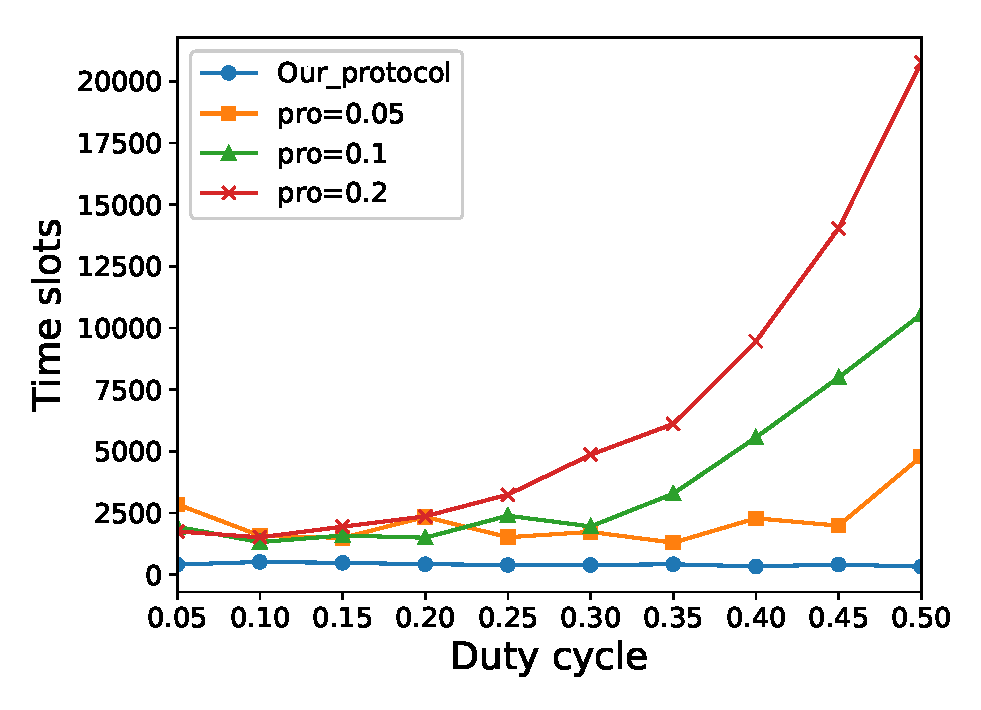
\includegraphics[width=1.65in]{figures/figure4.eps}}
    \caption{Time for encounter process increases when the duty cycle grows from $0.05$ to $0.5$.
    Figure~(a) depicts the slots for detecting stage and connecting stage of our protocol and figure~(b)
    compares our protocol with the three baseline methods.}
    \label{fig_DC}
\end{figure}

\begin{figure*}[!t]
    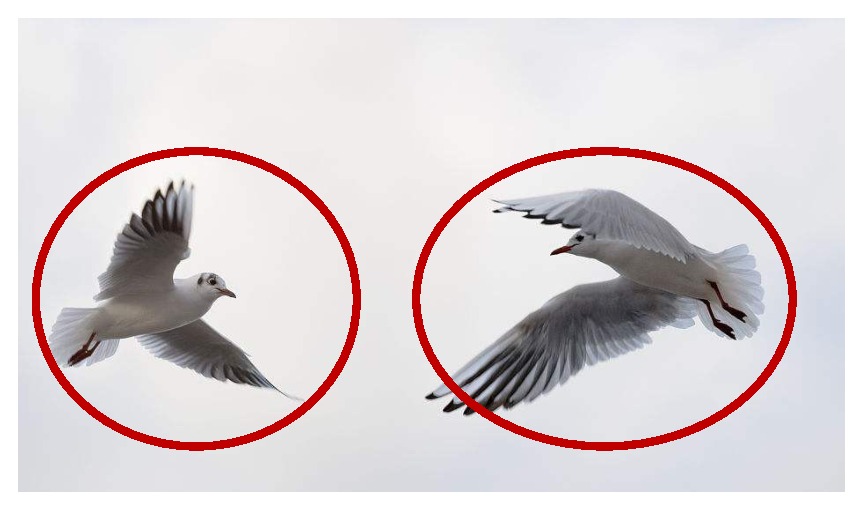
\includegraphics[width=.32\textwidth]{figures/AtoA}
    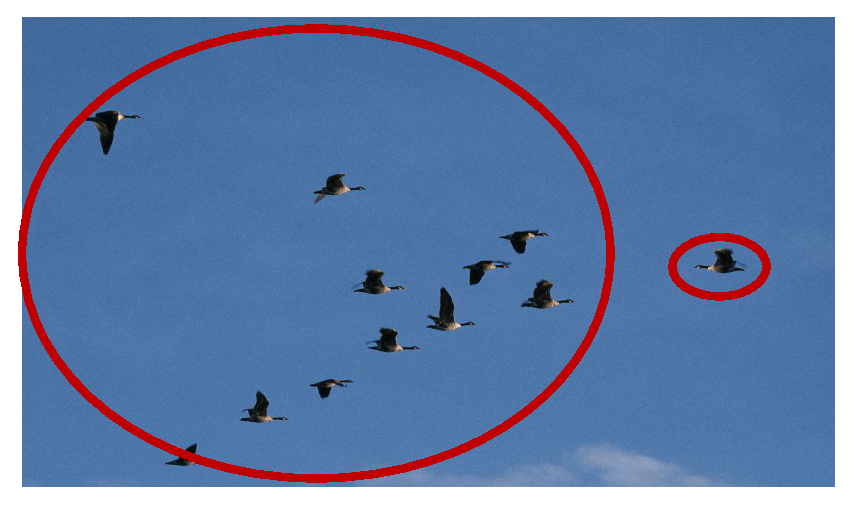
\includegraphics[width=.32\textwidth]{figures/AtoG}
    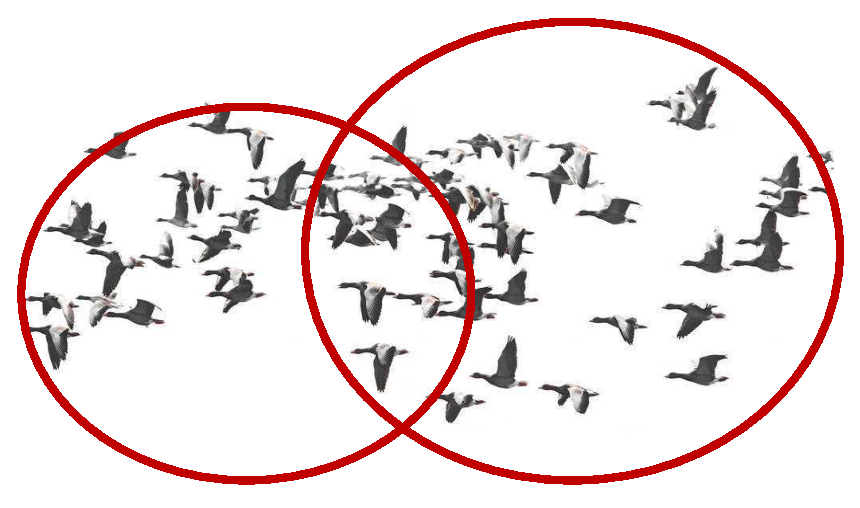
\includegraphics[width=.32\textwidth]{figures/GtoG}
    \caption{Encounter examples of three fundamental cases}
    \label{examples}
\end{figure*}

In Fig.~\ref{fig_DC}, we fix the the number of agents as $100$ and
increase duty cycle from $0.05$ to $0.5$. Fig.~\ref{fig_DC}~(a) show 
the time for encounter process of our protocol stays steady when duty cycle varies.
Particularly, the slots needed in the detecting stage decreases when duty cycle increases.
This is because higher duty cycle increases the probability that an agent is active in each slot.
Also we can see in Fig.~\ref{fig_DC}~(b) that the baseline methods
increase the latency as the duty cycle rises.

Next, we record the encounter registration rate in each time slot.
Encounter registration rate is defined as the proportion of agents that has been 
recorded. 

\begin{figure}[h]
    \centering
    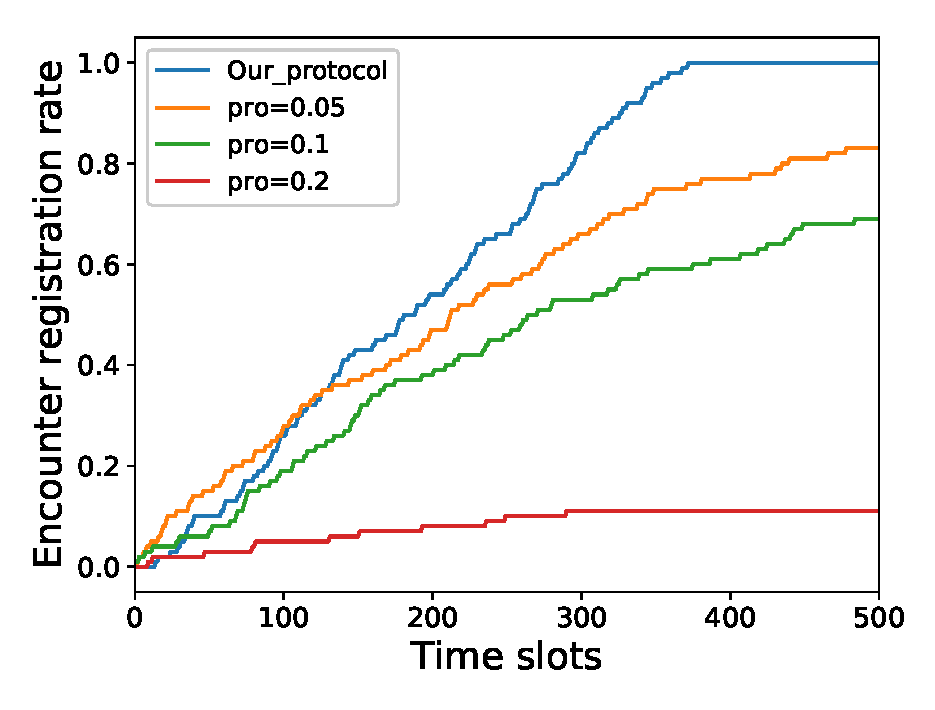
\includegraphics[width=3in]{figures/figure5.eps}
    \caption{Encounter process with $100$ agents and duty cycle of $0.25$. 
    Encounter registration rate increases as time goes on. Our protocol keeps
    the highest rate during the whole process.}
    \label{fig5}
\end{figure}

\begin{figure}[h]
    \centering
    \includegraphics[width=3in]{figures/figure6.eps}
    \caption{Encounter process with $100$ agents and duty cycle of $0.5$. 
    Encounter registration rate increases as time goes on. Our protocol keeps
    the highest rate during the whole process.}
    \label{fig6}
\end{figure}

We set the number of agents as $100$, and fix
duty cycle as $0.25$ in Fig.~\ref{fig5} and $0.5$ in Fig.~\ref{fig6}.
The same trend can be seen that our protocol has higher encounter registration rate
all the time and reaches to $1.0$ faster than the other methods.

In conclusion, our protocol outperforms the fixed transmitting probability methods 
and has better scalability. 

\subsection{Mobility}

The essential difference between a wildlife tracing system
and a mobile wireless network is the variability among the animal
species in their movement and interaction behavior.
The key challenge is that depending on the targeted animals, 
the moving speed and mobility might vary greatly, and 
the herd characteristics may also be very different.
%depending on the targeted animals. 

In this paper, we consider three explicit animal models of mobility
and build the simulation models as they relate to animal movement and interaction. 
This is the same approach that has been used in mobile wireless networks where 
human and vehicular mobility are characterized in a similar fashion.
%assigned rigorous underpinnings.
Specifically, we model their moving speeds as follows:
\begin{itemize}
    \item \textbf{Species I:} move at speed of $50$ m/s. 
    \item \textbf{Species II:} move at speed of $30$ m/s. 
    \item \textbf{Species III:} move at speed of $10$ m/s. 
\end{itemize}
Recall that the time length of a synchronized slot in reality 
is set as $20$~$ms$ and the radio range is set as $20$~$m$.

We evaluate our protocol in three simple and heuristic cases, as depicted in Fig.~\ref{examples}.
\begin{itemize}
    \item Case I: encounter for two agents, 
    e.g., two birds fly towards each other and then 
    fly apart, as depicted in Fig.~\ref{examples}~(a). 
    \item Case II: encounter for a single 
    agent with a group of agents, e.g., a bird fly into 
    a group of birds, as depicted in Fig.~\ref{examples}(b).
    \item Case III: encounter for two groups of agents, 
    e.g., two groups of birds fly towards each other and then fly 
    apart, as depicted in Fig.~\ref{examples}(c).
\end{itemize}

\begin{figure}[!h]
    \centering
    \includegraphics[width=3in]{figures/figure7.eps}
    \caption{Encounter for two agents. Our protocol
    achieves $100\%$ encounter registration rate.}
    \label{fig7}
\end{figure}

\subsubsection{Encounter for two agents}

We can see from Fig.~\ref{fig7} that both
agents employing our protocol can record each
other regarding all the three species.

\begin{figure}[!h]
    \centering
    \includegraphics[width=3in]{figures/figure8.eps}
    \caption{Encounter for a single 
    agent with a group of agents. Overall, our protocol
    achieves higher encounter registration rate.}
    \label{fig8}
\end{figure}

\subsubsection{Encounter for a single 
agent with a group of agents}

It can be seen from Fig.~\ref{fig8} that 
our protocol has higher encounter
registration rate (the proportion of agents that can 
be recorded by the single agent) than all the other methods.
Particularly, our protocol achieves nearly $100\%$ registration
rate regarding species II and species III.
This is because these two species move more slowly than species I 
so that the agents can be recorded in higher probabilities. 

\begin{figure}[!h]
    \centering
    \subfigure[]{\includegraphics[width=1.65in]{figures/figure9_A.eps}}
    \hspace{0.01in}
    \subfigure[]{\includegraphics[width=1.65in]{figures/figure9_B.eps}}
    \caption{Figure~(a) shows the proportion of agents in group A can 
    be recorded by the agents in group B, and Figure~(b) describes
    the opposite case. Overall, our protocol
    achieves higher encounter registration rate.}
    \label{fig9}
\end{figure}

\subsubsection{Encounter for two groups of agents}

Fig.~\ref{fig9}~(a) shows the proportion of agents in group A having 
been recorded by the agents in group B, and Fig.~\ref{fig9}~(b) depicts
the opposite case. Overall, our protocol achieves higher encounter 
registration rate than all the other methods. Particularly, species III
has higher encounter registration rate than species II and III.
This is because species III moves the most slowly and thus there are more 
chances for agents to detect and connect their peers. 

\section{Experiments for model validation}
\label{experiments}

We carried out a number of experiments in order to validate the radio model. 
All the experiments used LAUNCHXL-CC1350-4 evaluation boards with CC1350 RF microcontrollers by Texas Instruments.
We used a quiet frequency in the 434~MHz band, for which the boards are
designed, and the built-in helix antenna printed on the boards.
This antenna is fairly inefficient, resulting in about 4x to 8x degradation in communication range. 
% We used it because the shorter 
% ranges make testing easier
% and also because antennas on small wildlife tags tend to be inefficient due to the tiny ground plane.
% The chips that we tested are widely used in miniature wildlife tags,
% and they are a modern
% version of the chips that were used on the original Encounternet tags.
% requires more citations.

In all the tests we configured the radios for GFSK modulation, 500~kb/s, $\pm 250$~kHz deviation, 1243~kHz receive bandwidth,
and 10~dBm transmitting power. We used a Windows program called SmartRF Studio version~7 to drive the boards during
the tests and to log received packets. In all the tests,
a single board transmits 1.87~packets per second (intervals of
500~ms between packets). A packet consists of a 4-byte preamble, 4-byte sync workd, a length byte, 30-byte payload 
that includes a sequence number, and a 2-byte checksum. The fast transmission rate reduces power consumption (per byte and
per packet) and leads to short communication ranges, which is consistent with the goal of registering close encounters.

In a preliminary test, we configured one board to transmit packets, one
board to receive them, and a third one to transmit a
CW carrier at the same frequency. The three boards were at a distance of 0.4~m from each other. When the CW transmitter
was off, virtually all packets were received correctly. When the CW transmitter was on, virtually no packets were received.
This verifies that interference indeed blocks the receiver and may prevent packets from being received.
% It would have been good to transmit two packets simulteneously but there is no easy way to synchronize the boards.

% \begin{figure}[h]
%     \centering
%     \includegraphics[width=3in]{experiments/rssiHistograms.eps}
%     \caption{Histograms of the RSSI of received packets at different distances between 
%     the transmitter and the receiver. At the four distances reported in the figure, 
%     virtually all transmitted packets were received correctly.}
%     \label{fig:rssiHistograms}
% \end{figure}

% \begin{figure}[h]
%     \centering
%     \includegraphics[width=3in]{experiments/rssiDistance.eps}
%     \caption{Mean RSSI (after removal of outliers) at different distances, in black. 
%     The red curve is a least-square
%     fitting of the data to a 6~dB attenuation when the distance doubles.
%     The means shown in this figure are of the center 50\% of the packets; 
%     the extreme 50\% were filtered to remove outliers.}
%     \label{fig:rssiDistance}
% \end{figure}

\begin{figure}[h]
    \centering
    \subfigure[]{\includegraphics[width=1.65in]{figures/rssiHistograms.eps}}
    \hspace{0.01in}
    \subfigure[]{\includegraphics[width=1.4in]{figures/rssiDistance.eps}}
    \caption{Figure~(a) depicts RSSI of received packets at different distances between 
    the transmitter and the receiver. Figure~(b) describes mean RSSI at 
    different distances (the black curve) and a least-square
    fitting of the data to a 6~dB attenuation when the distance doubles
(the red curve).}
    \label{fig:rssi}
\end{figure}

In the main test, we placed the transmitter board at a fixed position, about 1.4~m above ground, and measured receive
performance at various distances between 2 and 78~m in an outdoor area with some human activity (but not much). We 
maintained each test position for at least 5 minutes.
The receiver board was also placed about 1.4~m above ground. In all the tests shown in graphs the transmit
and receive antennas were pointing at each other. We also performed a few tests with the receive antenna rotated 90~degrees;
RSSI values were about 1--2~dB lower but the overall results were similar; this is consistent with the characterization
of the antenna, which indicates that it is fairly omnidirectional.
The main results are shown in Figure~\ref{fig:rssi}~(a).
At each distance we measured the fraction of correctly-received packets and the RSSI of each packet. At the four
distances reported in the figure, virtually all transmitted packets were received correctly. We can see a clear
statistical correlation between distance and RSSI. Figure~\ref{fig:rssi}~(b) shows that the RSSI values
roughly follow the theoretical rule that stipulates a 6~dB attenuation when the distance doubles. The means
shown in this figure are of the center 50\% of the packets; the extreme 50\% were filtered to remove outliers.

We also tested performance at distances of 53~m and 78~m. At these distances, results were inconsistent. In one test
at 78~m, 84\% of the packets with mean RSSI of -98~dB. But in another test two hours later, only 2\% of the packets
were correctly received. At 53~m, no packets were received correctly for over 5 minutes. This location was in a depression,
about 3~m lower than both the transmitter and from the 78~m position; this may have contributed to the worse performance.
The main conclusion from these long-distance experiments (long given the bit rate) is that packets can sometimes be received
at fairly long distances and with RSSI values that typically characterize much shorter distances. 

However, the results also indicate that by dropping packets with low RSSI, say below -90~dB for these settings, we can
effectively limit the communication range to 20~m or so.

\section{Conclusions}
\label{sectionconclusion}
\vspace{-0.01in}
In this paper, we study the encounter registration problem in a single-hop network of $k$ 
agents. We propose a protocol consisting of two stages, namely detecting stage and 
connecting stage. Our protocol guarantees that, when an encounter happens, 
an agent in detecting stage will switch 
to the connecting stage very soon. After all the agents are in the connecting stage,  
each of them can record all the peers in $O(k)$ slots with high probability.
We present concrete analysis of the protocol under the radio model and validate the model 
by real-world experiments. 

\bibliographystyle{IEEEtran}
\bibliography{ref/ref.bib}

\end{document}

